%%%%%%%%%%%%%%%%%%%%%%%%%%%%%%%%%%%%%%%%%
% University/School Laboratory Report
% LaTeX Template
% Version 3.1 (25/3/14)
%
% This template has been downloaded from:
% http://www.LaTeXTemplates.com
%
% Original author:
% Linux and Unix Users Group at Virginia Tech Wiki 
% (https://vtluug.org/wiki/Example_LaTeX_chem_lab_report)
%
% License:
% CC BY-NC-SA 3.0 (http://creativecommons.org/licenses/by-nc-sa/3.0/)
%
%%%%%%%%%%%%%%%%%%%%%%%%%%%%%%%%%%%%%%%%%

%----------------------------------------------------------------------------------------
%	PACKAGES AND DOCUMENT CONFIGURATIONS
%----------------------------------------------------------------------------------------

\documentclass[a4paper]{article}

\usepackage[margin=1 in]{geometry}
\usepackage{listings}
\usepackage{graphicx} % Required for the inclusion of images
\usepackage{natbib} % Required to change bibliography style to APA
\usepackage{amsmath} % Required for some math elements 

%\setlength\parindent{0pt} % Removes all indentation from paragraphs

%\renewcommand{\labelenumi}{\alph{enumi}.} % Make numbering in the enumerate environment by letter rather than number (e.g. section 6)


%----------------------------------------------------------------------------------------
%	DOCUMENT INFORMATION
%----------------------------------------------------------------------------------------

\title{Final project report on \\Path Finding Problem \\~ \\ CS 7750} % Title

\author{Zolbayar Magsar \\Chanmann Lim \\Yihan Xu}

\date{December 15, 2014}

\begin{document}

\maketitle % Insert the title, author and date

\lstset{language=Java,title=\lstname,basicstyle=\footnotesize}

\begin{center}
Electrical \& Computer Engineering \\
University of Missouri, Columbia \\
\vspace{.5 in}
Instructor: Dr. Yi Shang \\
\end{center}

\vspace{1 in}

% If you wish to include an abstract, uncomment the lines below
\begin{abstract}
In many occasions, we face the problem of finding a path from one place to another place. In such situations, were we not just trying to find the shortest distance; but the traveling time also an important factor to be taken into consideration. In artificial intelligence, search algorithms are mainly used for such problems. On the other hand, when it comes to differentiating between such algorithms, it is often useful to implement them on a path finding problem and compare their features. We have attempted to create a game map which can be used in a simple path finding problem. On the map, we have two points, source and destination. We are also free to create an arbitrary shape of walls between them to create a problem. We then have myriad of ways to examine the precise difference between search algorithms and compare them in terms of execution speed, accuracy, and overall performance. To solve the path finding problem, we have implemented six major search algorithms representing 3 main types of search algorithm families, namely Breadth-First Search, Depth-First Search, Greedy Best-First Search, A* Search, Hill-Climbing, and Simulated Annealing. The map is created using a grid structure, so as to have a precise depiction of the 'search movements' of each of the algorithms visually in terms of characteristics and performance.
\end{abstract}

% \vfill

%----------------------------------------------------------------------------------------
%	SECTION 1
%----------------------------------------------------------------------------------------

\section{Introduction}

\emph{Pathfinding} or \emph{pathing} is the plotting, by a computer application, of the shortest route between two points. Two primary problems of pathfinding are to find a path between two nodes in a graph and to find the optimal shortest path. Basic algorithms such as Breadth-first and Depth-first search address the first problem by exhausting all possibilities; starting from the given node, they iterate over all potential paths until they reach the destination node. The more complicated problem is finding the optimal path. However, it is not necessary to examine all possible paths to find the optimal one. Algorithms such as A* strategically eliminate paths, through heuristics while local search such as Hill-climbing further reduce search space to a constant number of choices to make search rocket fast.\\

\noindent At its core, a pathfinding method searches a graph by starting at one vertex and exploring adjacent nodes until the destination node is reached, generally with the intent of finding the shortest route. Although graph searching methods such as a Breadth-first search would find a route if given enough time, other methods, which "explore" the graph, would tend to reach the destination sooner. An analogy would be a person walking across a room; rather than examining every possible route in advance, the person would generally walk in the direction of the destination and only deviate from the path to avoid an obstruction, and make deviations as minor as possible.\\

\noindent We have implemented six different algorithms to traverse and find the pathway on a grid from a given square A to destination B using 3 main strategies of search algorithms:\\

\begin{enumerate}
\item Uninformed search
	\begin{itemize}
		\item Breath-first search
		\item Depth-first search
	\end{itemize}
\item Heuristic search
	\begin{itemize}
		\item Greedy best-first search
		\item A* search
	\end{itemize}
\item Local search
	\begin{itemize}
		\item Hill-climbing
		\item Simulated annealing
	\end{itemize}
\end{enumerate}

% \subsection{Definitions}
% \label{definitions}
% \begin{description}
% \item[Stoichiometry]
% The relationship between the relative quantities of substances taking part in a reaction or forming a compound, typically a ratio of whole integers.
% \item[Atomic mass]
% The mass of an atom of a chemical element expressed in atomic mass units. It is approximately equivalent to the number of protons and neutrons in the atom (the mass number) or to the average number allowing for the relative abundances of different isotopes. 
% \end{description} 
 
%----------------------------------------------------------------------------------------
%	SECTION 2
%----------------------------------------------------------------------------------------

\section{Algorithms and Implementations}

There will be obstacles between A and B, and our implementation would show graphically how the algorithm manage to reach the destination, which in turn would visually demonstrate the actual performance of algorithms in real world problems. We made use of Manhattan distance as the heuristics for the informed search algorithms and as the scoring function for local searches.

%----------------------------------------------------------------------------------------
%	Breadth-first
%----------------------------------------------------------------------------------------

\subsection{Breadth-first search algorithm:}

BFS is a  strategy for searching in a graph  when search is limited to essentially two operations: (a) visit and inspect a node of a graph; (b) gain access to visit the nodes that neighbor the currently visited node. The BFS begins at a root node and inspects all the neighboring nodes. Then for each of those neighbor nodes in turn, it inspects their neighbor nodes which were unvisited, and so on. \\

\begin{figure}[h!]
  \centering
    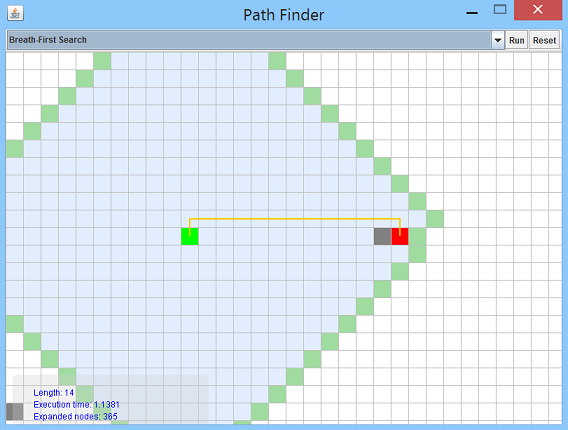
\includegraphics[scale=.9]{images/bfs1.png}
  \caption{BFS with a block between two points}
\end{figure}

\noindent \\
The algorithm uses a queue data structure to store intermediate results as it traverses the graph, as follows:\\

\begin{enumerate}
\item Enqueue the root node
\item Dequeue a node in first-in-first-out manner and examine it
	\begin{itemize}
		\item If the element sought is found in this node, quit the search and return a result.
		\item Otherwise enqueue any successors (the direct child nodes) that have not yet been discovered.
	\end{itemize}
\item If the queue is empty, every node on the graph has been examined – quit the search and return "not found". \\
\item If the queue is not empty, repeat from Step 2.
\end{enumerate}

%----------------------------------------------------------------------------------------
%	Depth-first
%----------------------------------------------------------------------------------------

\subsection{Depth-first search algorithm:}

DFS starts at the root (selecting some arbitrary node as the root in the case of a graph) and explores as far as possible along each branch before backtracking. \\

\begin{figure}[h!]
  \centering
    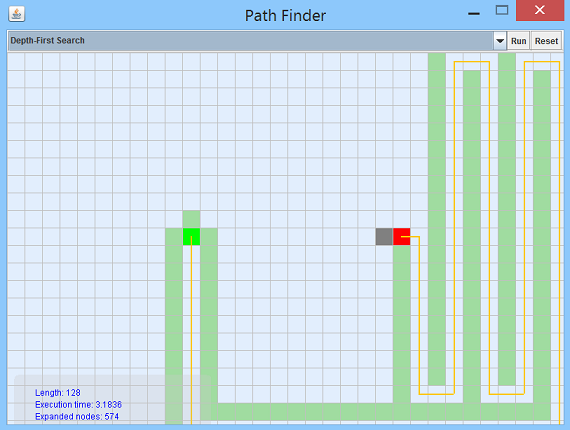
\includegraphics[scale=.9]{images/dfs1.png}
  \caption{DFS with a block between two points}
\end{figure}

\noindent \\
DFS always expands the deepest node in the current frontier of the search tree. As seen above, the search proceeds immediately to the deepest level of the search tree, where the nodes have no successors.

%----------------------------------------------------------------------------------------
%	Greedy best-first
%----------------------------------------------------------------------------------------

\subsection{Best-first search algorithm:}

It is a search algorithm which explores a graph by expanding the most promising node chosen according to a specified rule.\\

\noindent We used "best-first search" to refer specifically to a search with a  heuristic function that attempts to predict how close the end of a path is to a solution, so that paths which are judged to be closer to a solution are extended first. This specific type of search is called \textbf{greedy best-first search}. \\

\begin{figure}[h!]
  \centering
    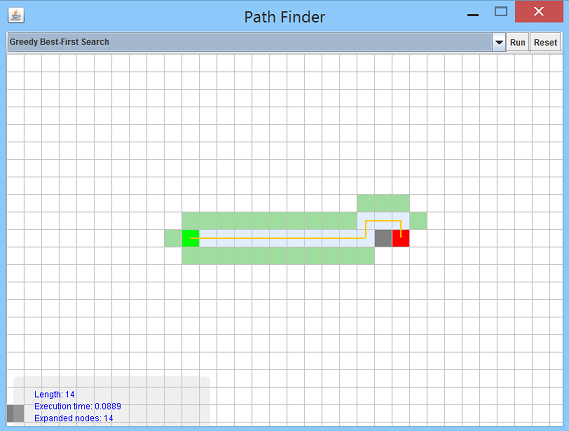
\includegraphics[scale=.9]{images/greedy1.png}
  \caption{Greedy best-first search with a block between two points}
\end{figure}

\noindent \\
By using a greedy algorithm, we expand the first successor of the parent. After a successor is generated: \\
\begin{enumerate}
	\item If the successor's heuristic is better than its parent, the successor is set at the front of the queue (with the parent reinserted directly behind it), and the loop restarts.
	\item Else, the successor is inserted into the queue (in a location determined by its heuristic value). The procedure will evaluate the remaining successors (if any) of the parent.
\end{enumerate}

%----------------------------------------------------------------------------------------
%	A*
%----------------------------------------------------------------------------------------

\subsection{A* search algorithm:}

A* assigns a weight to each open node equal to the weight of the edge to that node plus the approximate distance between that node and the finish. This approximate distance is found by the heuristic, and represents a minimum possible distance between that node and the end. This allows it to eliminate longer paths once an initial path is found. If there is a path of length x between the start and finish, and the minimum distance between a node and the finish is greater than x, that node need not be examined. \\

\begin{figure}[h!]
  \centering
    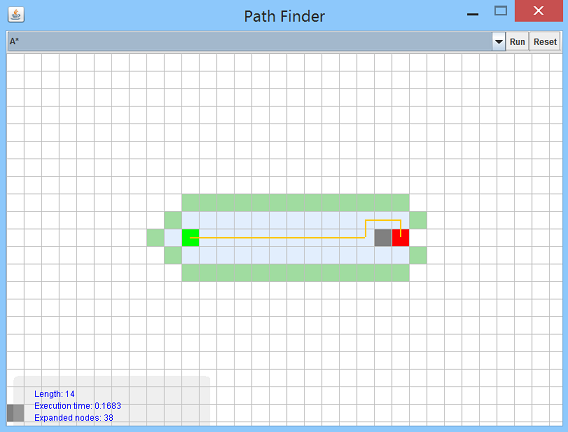
\includegraphics[scale=.9]{images/A1.png}
  \caption{A* with a block between two points}
\end{figure}

\noindent \\
When the value of the heuristic is exactly the true distance, A* examines the fewest nodes. As the value of the heuristic increases, A* examines fewer nodes but no longer guarantees an optimal path. In many applications (such as video games) this is acceptable and even desirable, in order to keep the algorithm running quickly.

%----------------------------------------------------------------------------------------
%	Hill-climbing
%----------------------------------------------------------------------------------------

\subsection{Hill-climbing algorithm:}

A local search algorithm starts from a candidate solution and then iteratively moves to a neighbor solution. When no improving configurations are present in the neighborhood, local search is stuck at a locally optimal point. \\

\begin{figure}[h!]
  \centering
    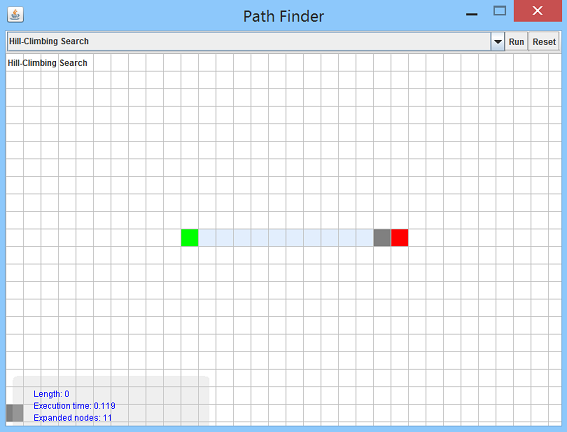
\includegraphics[scale=.9]{images/hillclimb1.png}
  \caption{Hill-climbing search with a block between two points}
\end{figure}

\noindent \\
It is an iterative algorithm that starts with an arbitrary solution to a problem, then attempts to find a better solution by incrementally changing a single element of the solution. If the change produces a better solution, an incremental change is made to the new solution, repeating until no further improvements can be found. Hill climbing is good for finding a local optimum (a solution that cannot be improved by considering a neighboring configuration) but it is not necessarily guaranteed to find the best possible solution (the global optimum) out of all possible solutions (the search space).

%----------------------------------------------------------------------------------------
%	Simulated annealing
%----------------------------------------------------------------------------------------

\subsection{Simulated annealing algorithm:}

At each step, the SA heuristic considers some neighboring state of the current state, and probabilistically decides between moving the system to that state or staying in the current state. These probabilities ultimately lead the system to move to states of lower energy. Typically this step is repeated until the system reaches a state that is good enough for the application, or until a given computation budget has been exhausted. \\

\begin{figure}[h!]
  \centering
    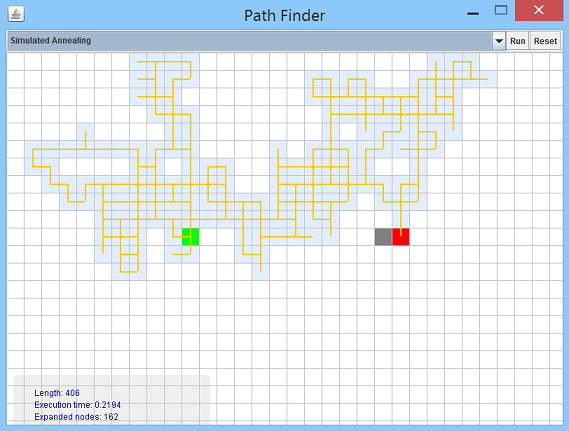
\includegraphics[scale=.9]{images/sa1.png}
  \caption{Simulated annealing with a block between two points}
\end{figure}

\noindent \\
The innermost loop of the simulated-annealing algorithm is quite similar to hill climbing. Instead of picking the best move, however, it picks a random move. If the move improves the situation, it is always accepted. Otherwise, the algorithm accepts the move with some probability less than 1.

\paragraph{Use of grids:} Grids are commonly used in games for representing playing areas such as maps (in games like Civilization and Warcraft), playing surfaces (in games like pool, table tennis, and poker), playing fields (in games like baseball and football), boards (in games like Chess, Monopoly, and Connect Four), and abstract spaces (in games like Tetris). \\

\begin{figure}[h!]
  \centering
    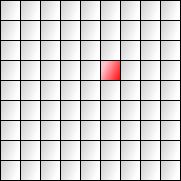
\includegraphics[scale=.6]{images/square-grid.png}
  \caption{Square grida}
\end{figure}

\noindent Grids are built from a repetition of simple shapes. The most common grid is a square grid. It’s simple, easy to work with, and maps nicely onto a computer screen. Square grids are the most common grids used in games, primarily because they are easy to use. Locations can use the familiar cartesian coordinates (x, y) and the axes are orthogonal. The square coordinate system is the same even if your map squares are angled on screen in an isometric or axonometric projection.

%----------------------------------------------------------------------------------------
%	SECTION 3
%----------------------------------------------------------------------------------------

\section{Results and Analysis}

The results we have obtained, after running these algorithms individually both with and without a block between the points A and B, are pretty astonishing and is a pleasure for anyone to watch how these algorithms get the job done through such distinctive methodologies.\\

\noindent Let us compare the six algorithms in an exactly same problem case with a single square block in between the two points.

\begin{figure}[h!]
  \centering
    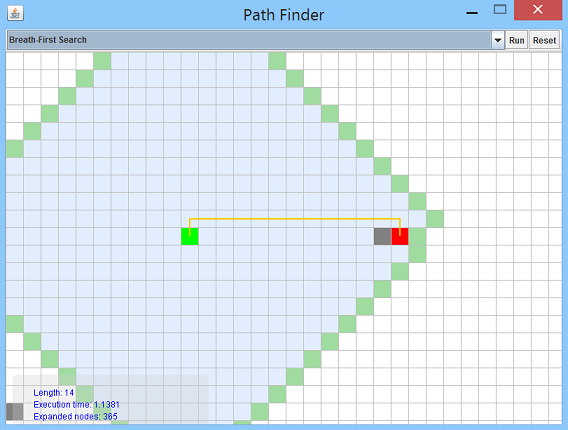
\includegraphics[scale=.9]{images/bfs1.png}
  \caption{BFS with a block between two points}
\end{figure}

\noindent As we can see here, in breadth-first search algorithm, all the nodes are expanded at a given depth in the search tree before any nodes at the next level are expanded. Therefore the shape of the search space covered is guaranteed to be a square on a grid and the expanded node is the largest in case of BFS. The CPU execution time is also the longest since the algorithm is doing an exhaustive search to reach the destination node. We can see how blind (and wasteful) an uninformed search actually is. Breadth-first search is guaranteed to find the optimal path, so we can see that the path-cost is 14 in above case. \\

\begin{figure}[h!]
  \centering
    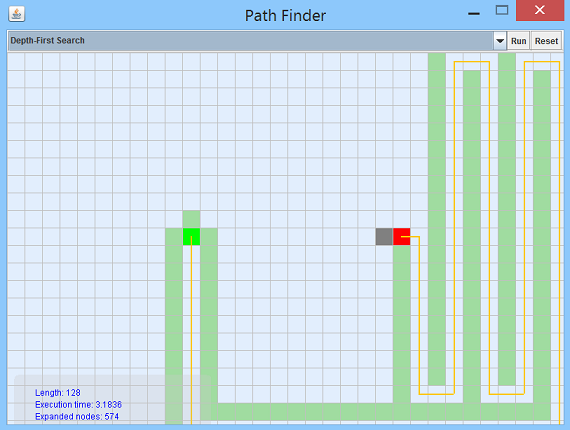
\includegraphics[scale=.9]{images/dfs1.png}
  \caption{DFS with a block between two points}
\end{figure}

\noindent As we can see here, DFS expands the deepest node in the current frontier. Therefore the path cost is quite high in this example and the CPU execution time as well. It also expanded much more nodes than BFS, therefore proving that DFS is non-optimal. \\

\begin{figure}[h!]
  \centering
    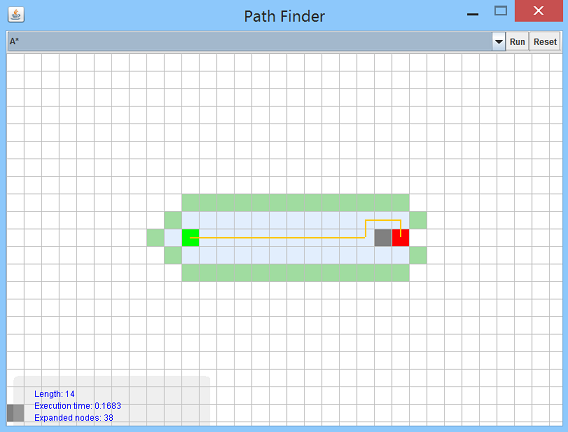
\includegraphics[scale=.9]{images/A1.png}
  \caption{A* with a block between two points}
\end{figure}

\noindent We can see from the above picture how smart the heuristic search compared to the uninformed search is. A* actually has a sense of direction to look for the destination and is very effective in finding it. The length of the path is same as BFS, therefore guarantees an optimal path, because of an admissible heuristic function. We can see that the expanded node is greatly reduced and the CPU execution time accordingly. \\

\begin{figure}[h!]
  \centering
    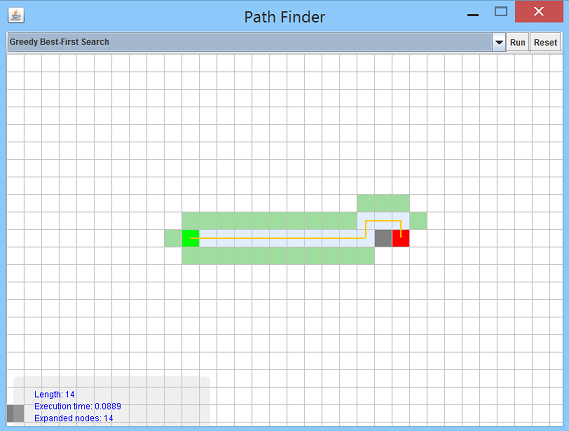
\includegraphics[scale=.9]{images/greedy1.png}
  \caption{Greedy best-first search with a block between two points}
\end{figure}

\noindent The greedy best-first search is the most effective in this case with a minimum expanded nodes of 14, thereby having the least CPU execution time. This proves that a greedy algorithm can be very effective in the right circumstance. Instead of selecting the vertex closest to the starting point, it selects the vertex closest to the goal. Greedy Best-First-Search is not guaranteed to find a shortest path. However, it runs much quicker than A* algorithm. \\

\begin{figure}[h!]
  \centering
    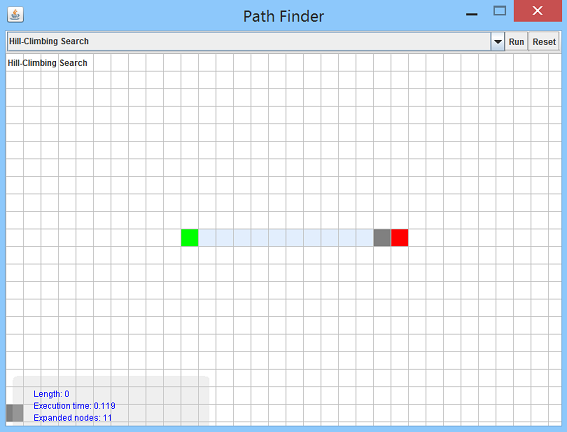
\includegraphics[scale=.9]{images/hillclimb1.png}
  \caption{Hill-climbing search with a block between two points}
\end{figure}

\noindent As we can see (in Figure 6), a local search algorithm operate using a single current node (rather than multiple paths) and generally move only to neighbors of that node. Also the paths followed by the search are not retained. So we can testify from above that the hill-climbing search is simply a loop that continually moves in the direction of increasing value – that is, uphill. And since there’s an obstacle, it failed to find the path to the destination, because it simply did not keep track of alternative routes. Hence we can see the clear limitations of the hill-climbing search here. \\

\begin{figure}[h!]
  \centering
    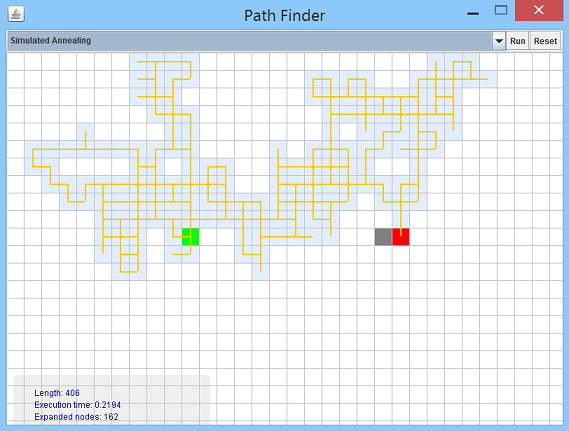
\includegraphics[scale=.9]{images/sa1.png}
  \caption{Simulated annealing with a block between two points}
\end{figure}

\noindent Simulated annealing is the most ineffective choice as per this example as the path length is 406 steps as shown. However, the CPU execution time and the expanded node are much less than uninformed search algorithms because of its randomness.


%----------------------------------------------------------------------------------------
%	SECTION 4
%----------------------------------------------------------------------------------------

\section{Conclusion}

So the obvious question is "which algorithm should we use for finding paths on a game map?"

\begin{itemize}
\item If you want to find paths from or to all locations, use Breadth First Search.
\item If you want to find paths to one location, use Greedy Best First Search or A*. We would prefer A* in most cases since it is optimal.
\end{itemize}

\noindent What about optimal paths? Breadth First Search is guaranteed to find the shortest path given the input graph. Greedy Best First Search is not. A* is guaranteed to find the shortest path if the heuristic is never larger than the true distance. As the heuristic becomes larger, A* turns into Greedy Best First Search.\\

\noindent What about performance? The best thing to do is to eliminate unnecessary locations in your graph. Reducing the size of the graph helps all the graph search algorithms. It also can be noticed that simpler queues run faster. Greedy Best First Search typically runs faster but doesn’t produce optimal paths. A* is a good choice for most pathfinding needs.

\newpage

%$T_k = \frac{T_0}{1 + \alpha \cdot k}, \quad \alpha > 0$

%----------------------------------------------------------------------------------------
%	BIBLIOGRAPHY
%----------------------------------------------------------------------------------------

%\bibliographystyle{apalike}

%\bibliography{sample}

%----------------------------------------------------------------------------------------


\end{document}